\section{Caltrans Bridge No. 04-0236} %{CE89324} Painter St
\label{sec:painter}

\begin{figure}[H]
    \centering
    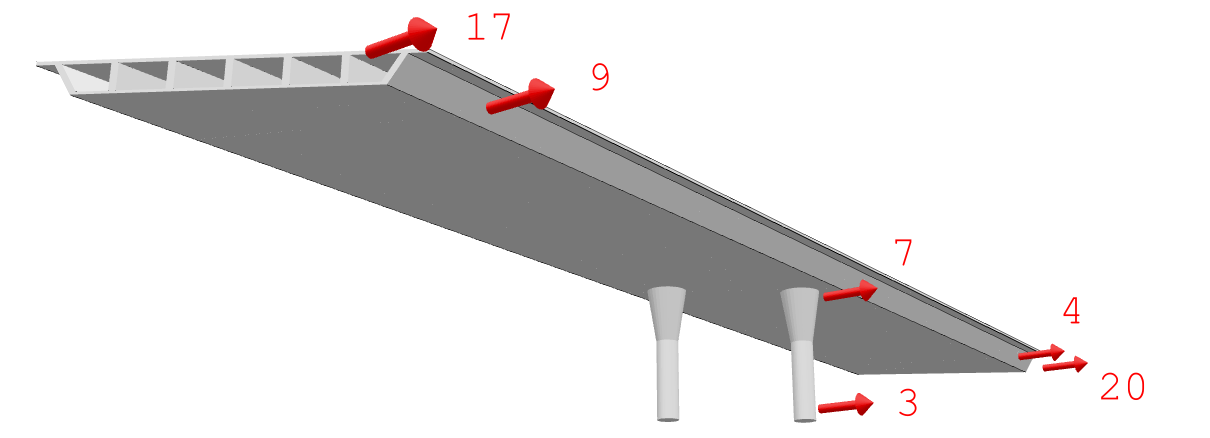
\includegraphics[width=0.8\textwidth]{Examples/04-0236/about/painter_sensors_labels.png}
    \caption{Accelerometer placement on the Painter St. Overpass. Adapted from \cite{chern2025evaces}.}
    \label{fig:painter_instrumentation}
\end{figure}

\subsection{Introduction}

The US 101/Painter St. Overpass is a continuous reinforced concrete box-girder bridge, \cref{fig:painter-warping}. 
The skewed 265-foot-long deck consists of
two unequal spans which meet at a two-column bent. 
The 40-foot-wide roadway accommodates one traffic lane in each direction, each with a
comfortable shoulder. 
There is no horizontal or vertical curvature to the structure. 
The structure sits on two skewed integral abutments and
two column footings supported on 20 piles each.

The east abutment is monolithic with the superstructure and is supported
by 14 driven 45-ton concrete friction piles. 
The west abutment has a thermal expansion joint and rests on a neoprene bearing strip. 
The foundation of this abutment consists of 16 driven 45-ton concrete
friction piles. 
Continuous flared columns use an obsolete detail. 
An experimental investigation on this matter was conducted by \cite{sanchez1997seismic}. 
A numerical investigation of the continuous detail is conducted by \cite{soleimani2017seismic}. 
This issue is addressed by \textcite{caltrans2009memo-6-1}.

\subparagraph{Instrumentation and System Identification}

The Painter St. Overpass was instrumented in 1977. 
The bridge has recorded accelerations from a total of 22 strong motion events. 
The details of these events, including dates, times, and the \emph{peak station acceleration} (PSA) --- the maximum acceleration recorded at any accelerometer --- are listed in Table~\ref{tab:errors_identity}. 


\begin{table}[h]
    \centering
    \caption{
    Events recorded at the Painter St. Overpass (\texttt{CE89324}).}
    \begin{tabular}{ccc}
    \toprule
    Event & Date/Time & PSA (g)  \\
    \midrule
    0   &  2021-12-20T21:53:00  & 0.031  \\ %& 0.260 & 0.204 & 0.369 \\
    1   &  2016-12-08T14:50:00  & 0.031  \\ %& 0.319 & 0.255 & 0.336 \\
    2   &  2021-12-23T03:28:00  & 0.033  \\ %& 0.413 & 0.388 & 0.478 \\
    3   &  2023-05-21T18:44:00  & 0.034  \\ %& 0.334 & 0.165 & 0.431 \\
    4   &  2023-09-30T17:16:00  & 0.038  \\ %& 0.291 & 0.305 & 0.583 \\
    5   &  2022-12-20T15:08:00  & 0.052  \\ %& 0.375 & 0.347 & 0.642 \\
    6   &  2020-03-09T02:59:00  & 0.055  \\ %& 0.399 & 0.298 & 0.475 \\
    7   &  2022-04-04T15:16:00  & 0.056  \\ %& 0.313 & 0.307 & 0.515 \\
    8   &  2014-10-19T14:23:00  & 0.062  \\ %& 0.502 & 0.554 & 0.747 \\
    9   &  2023-08-17T21:07:00  & 0.064  \\ %& 1.136 & 1.098 & 0.999 \\
    10  &  2012-09-14T18:19:00  & 0.074  \\ %& 0.511 & 0.401 & 0.580 \\
    11  &  2023-10-16T10:20:00  & 0.089  \\ %& 0.298 & 0.373 & 0.598 \\
    12  &  2013-10-11T23:05:00  & 0.090  \\ %& 0.275 & 0.291 & 0.416 \\
    13  &  2022-12-20T10:38:00  & 0.143  \\ %& 0.466 & 0.959 & 0.754 \\
    14  &  2023-09-30T15:26:00  & 0.144  \\ %& 0.425 & 0.350 & 0.768 \\
    15  &  2016-12-05T18:32:00  & 0.169  \\ %& 0.734 & 0.635 & 0.890 \\
    16  &  2012-09-14T11:53:00  & 0.224  \\ %& 0.599 & 0.795 & 0.803 \\
    17  &  2019-06-23T03:52:00  & 0.248  \\ %& 0.277 & 0.273 & 0.388 \\
    18  &  2015-01-28T21:08:00  & 0.291  \\ %& 0.288 & 0.297 & 0.534 \\
    19  &  2024-12-05T18:44:00  & 0.565  \\ %& 0.379 & 0.454 & 0.617 \\
    20  &  2023-01-01T18:34:00  & 1.033  \\ %& 0.443 & 0.411 & 0.539 \\
    21  &  2022-12-20T10:34:00  & 1.384  \\ %& 0.616 & 0.659 & 0.839 \\
    \bottomrule
    \end{tabular}
    \label{tab:errors_identity}
\end{table}

Event 21, with a PSA of $1.38$ g, is notable for its intensity. 
Following this event, Caltrans conducted an on-site inspection, augmented by unmanned aerial vehicles, and identified the following damage \citep{heninger_use_2023}:
\begin{itemize}
    \item minor concrete cover spalling,
    \item shear key cracking, and
    \item a vertical displacement of approximately $1$ inch at the south (acute) corner of the east abutment.
\end{itemize}
No additional significant displacement or damage was observed.

%

% \begin{figure}[h!]
% \centering
% \includegraphics[trim={0 1.3cm 0 2.5cm},clip,width=0.7\textwidth]{figures/painter/ll89324_1}
% \caption{Instrumentation of the Painter Street Overpass.}\label{fig:painter-instrumentation}
% \end{figure}
% \begin{figure}[h!]
% \centering
% \includegraphics[trim={0 1.3cm 0 2.5cm},clip,width=\textwidth]{figures/painter-plot-3-7_notext.png}
% \caption{Historical transfer function estimates of 29 events for the Painter
% St.~Overpass (transverse direction using Channels 3 vs. 7). Event dates range between 1980 and 2023 with peak station accelerations ranging between $0.1g$ and $0.63g$.}\label{fig:painter-stfe}
% \end{figure}

% \begin{figure}
% \hypertarget{fig:painter-column}{%
% \centering
% 
\includegraphics{figures/painter-column-dwg.png}
% \caption{Lower section view of the typical bent
% column}\label{fig:painter-column}
% }
% \end{figure}

Various system identification studies have been conducted by the \BRACE{} team and results of several historical transfer function estimates are
provided in \cref{fig:painter-stfe}. 


\subparagraph{Literature}
\cite{maroney1990interpretation} utilized records from this Painter Street Overpass
in conjunction with a number of finite-element and lumped-parameter
(stick) models of the entire bridge. 
However, none of these models
accounted for soil-foundation-superstructure interaction. At each
abutment, soil-wall interaction was modeled through a single real-valued
transverse spring, the stiffness of which was inversely determined from the
interpreted fundamental natural period, \(T \approx 0.30\) seconds, in
lateral vibration.
%
\textcite{goel1997evaluation} identified the following abutment
stiffness parameters for two excitation intensities:
%
\begin{table}[H]
\centering
\begin{tabular}{lll}
\toprule
{\bf{Excitation}} & {\bf{Lower bound (kips/ft)}} & {\bf{Upper bound (kips/ft)}} \\
\midrule
%\endhead
Longitudinal (low intensity) & 11,000 & 13,115 \\
Transverse (high intensity) & 7,500 & 12,000 \\
\bottomrule
\end{tabular}
\end{table}

Additional studies whose findings have been worked into the
parameterization and calibration of the Painter Street models are those of
\textcite{zhang2002seismic} and \textcite{arici2003system}.
%%%\clearpage 
Other system identification and modeling studies have been performed and consistent identification of a fundamental period of about 0.29 seconds and a secondary period of about 0.23 seconds have been obtained and verified \cite{fraino_seismic_2012,safak_use_1994,turek_ambient_2014,mosquera2009utilization,ventura_dynamic_nodate,mccallen1994dynamic}.

% %
% \begin{figure}
% \hypertarget{fig:goel1997evaluation-model}{%
% \centering
% \includegraphics{figures/painter/goel1997evaluation-model.png}
% \caption{Model employed by
% \textcite{goel1997evaluation}}\label{fig:goel1997evaluation-model}
% }
% \end{figure}

% \begin{table}[h]
%     \centering
%     \input{tables/painter-instrumentation}
% \end{table}


%%%%%%%%%%%%%%%%%%%%\clearpage
% \begin{figure}
% \hypertarget{fig:painter-transverse}{%
% \centering
% 
\includegraphics{figures/painter/painter-transverse.pdf}
% \caption{Transverse mode for the M1 model of the Painter street
% overpass}\label{fig:painter-transverse}
% }
% \end{figure}

\begin{figure}[H]
\hypertarget{fig:painter-warping}{%
\centering
% 
\includegraphics[trim={0 1.3cm 0 1.3cm},clip,width=0.8\linewidth]{figures/painter-girder-mesh}
\caption{Finite element model used to obtain warping
shapes of US 101/Painter St. Overpass.}\label{fig:painter-warping}
}
\end{figure}

\iffalse
\subsection{Old}
The US 101/Painter street overpass is a continuous reinforced concrete
multicell box-girder bridge. 
The skewed 265 foot long deck consists of
two unequal spans which meet at a two-column bent. 
The 40 foot wide
roadway accommodates one lane of traffic in each direction, each with a
comfortable shoulder. 
There is no horizontal or vertical curvature to
the structure. The structure sits on two skewed integral abutments and
two column footings resting on 20 piles each.

\subparagraph{Abutments}

The east abutment is monolithic with the superstructure and is supported
by 14 driven 45-ton concrete friction piles. The west abutment meets at
a thermal expansion joint and rests on a neoprene bearing strip. The
foundation of this abutment consists of 16 driven 45-ton concrete
friction piles.

\subparagraph{Details}
Some details that should be noted about this bridge include:

\begin{itemize}
\tightlist
\item
  Continuous flared columns use obsolete detail An experimental
  investigation was conducted by \textcite{sanchez1997seismic} . A
  numerical investigation of the continuous detail is conducted by
  \textcite{soleimani2017seismic}. This issue is addressed by
  \textcite{caltrans2009memo-6-1}.
\end{itemize}

\begin{figure}
\hypertarget{fig:painter-warping}{%
\centering
% 
\includegraphics{figures/painter-girder-mesh.svg}
\caption{Finite element model used to obtain warping
constant.}\label{fig:painter-warping}
}
\end{figure}

\begin{figure}
\hypertarget{fig:painter-column}{%
\centering
% 
\includegraphics{figures/painter-column-dwg.png}
\caption{Lower section view of the typical bent
column}\label{fig:painter-column}
}
\end{figure}


\subparagraph{Instrumentation}

The Painter street overpass was instrumented in 1977.

% \begin{table}[h]
%     \centering
%     \input{tables/painter-instrumentation}
% \end{table}

\begin{figure}
\hypertarget{fig:painter-instrumentation}{%
\centering
% \includegraphics{figures/painter/ll89324_1.png}
\caption{Instrumentation of the Painter Street
Overpass}\label{fig:painter-instrumentation}
}
\end{figure}

\subsection{Literature}

\cite{maroney1990interpretation} utilized records from the Painter street overpass
in conjunction with a number of finite-element and lumped-parameter
(stick) models of the entire bridge. However, none of these models
accounted for soil-foundation-superstructure interaction. At each
abutment, soil-wall interaction was modeled through a single real-valued
transverse spring, the stiffness of which was backfigured from the
interpreted fundamental natural period, \(T \approx 0.30 \text{s}\), in
lateral vibration.

% \textcite{goel1997evaluation} identified the following abutment
% stiffness parameters for two excitation intensities:


% \begin{longtable}[]{@{}lll@{}}
% \toprule
% Excitation & Lower bound (kips/ft) & Upper bound (kips/ft) \\
% \midrule
% \endhead
% Longitudinal (low intensity) & 11,000 & 13,115 \\
% Transverse (high intensity) & 7,500 & 12,000 \\
% \bottomrule
% \end{longtable}


\begin{figure}
\hypertarget{fig:goel1997evaluation-model}{%
\centering
% \includegraphics{figures/painter/goel1997evaluation-model.png}
\caption{Model employed by
\textcite{goel1997evaluation}}\label{fig:goel1997evaluation-model}
}
\end{figure}

Additional studies whose findings have been worked into the
parameterization and calibration of the Painter St.~models are those of
\textcite{zhang2001seismic} and \textcite{arici2003system}.

\subsection{Analysis}
\subparagraph{System ID}
Various system identification studies have been conducted by the BRACE2
team, and results of several historical transfer function estimates are
provided in \ref{fig:painter-stfe}. 

\begin{figure}
\hypertarget{fig:painter-stfe}{%
\centering

\includegraphics{Part III/Figures/painter-plot-3-7.pdf}
\caption{Historical transfer function estimates of the Painter
St.~Overpass.}
\label{fig:painter-stfe}
}
\end{figure}

\section{Modeling}

\begin{figure}
\hypertarget{fig:painter-transverse}{%
\centering
% 
\includegraphics{figures/painter/painter-transverse.pdf}
\caption{Transverse mode for the M1 model of the Painter street
overpass}\label{fig:painter-transverse}
}
\end{figure}

\subsection{M1 Model}

The superstructure is modeled using traditional linear-elastic frame
elements with gross section properties.

The sole bent is modeled as a stiff beam framing into the
superstructure. Columns are linear-elastic, and rest on a flexible
foundation model consisting of linear springs.

Framing of the columns into the bent is modeled using a rigid joint
offset to account for the rigidity of the both the box girder, and
column flares which are notably built-in.

The abutments are modeled by a collection of parameterized linear
springs. Initial stiffness values can be selected from those reported in
the literature.

Mass is assigned to the structure using consistent mass distribution in
the frame elements.

\hypertarget{m2}{%
\subsection{M2}\label{m2}}

\hypertarget{m3}{%
\subsection{M3}\label{m3}}

\hypertarget{analysis}{%
\section{Analysis}\label{analysis}}

\hypertarget{a1---modal-analysis}{%
\subsection{A1 - Modal Analysis}\label{a1---modal-analysis}}

\hypertarget{a2---instrumentation-response-history}{%
\subsection{A2 - Instrumentation Response
History}\label{a2---instrumentation-response-history}}

Channels which may be considered for transverse excitation include 7, 9,
17 and 20. Longitudinal field channels include 11, 15 and 18.

\fi